\chapter{Chapter 1: Introduction to IoT}

This chapter compiles lecture-quality study notes and comprehensive exam answers for \textbf{Unit I: Introduction} of the OE-EC803A syllabus, adhering strictly to the \textbf{MAKAUT Answer Writing Guidelines}.


\section{Section 1: Definitions and Core Concepts (Q1.1)}

\subsection{1. Definition of Internet of Things (IoT)}
The \textbf{Internet of Things (IoT)} is a dynamic global network infrastructure with self-configuring capabilities based on standard and interoperable communication protocols. It connects physical and virtual \textbf{"things"} embedded with sensors, actuators, microcontrollers, and communication interfaces, allowing them to gather, process, and exchange data with minimal human intervention.

\subsection{2. WWW vs. IoT Comparison}
\begin{itemize}
  \item   \textbf{World Wide Web (WWW):} Connects \textbf{humans to information} using web browsers and standard protocols (HTTP/HTTPS) to access documents, web pages, and multimedia. It is a human-centric information network.
  \item   \textbf{Internet of Things (IoT):} Connects \textbf{devices to devices (things to things)}. It links physical objects, sensors, and actuators to exchange machine-generated data, trigger actions, and automate workflows. It is a machine-centric, physical-digital network.
\end{itemize}

\begin{figure}[H]
\centering
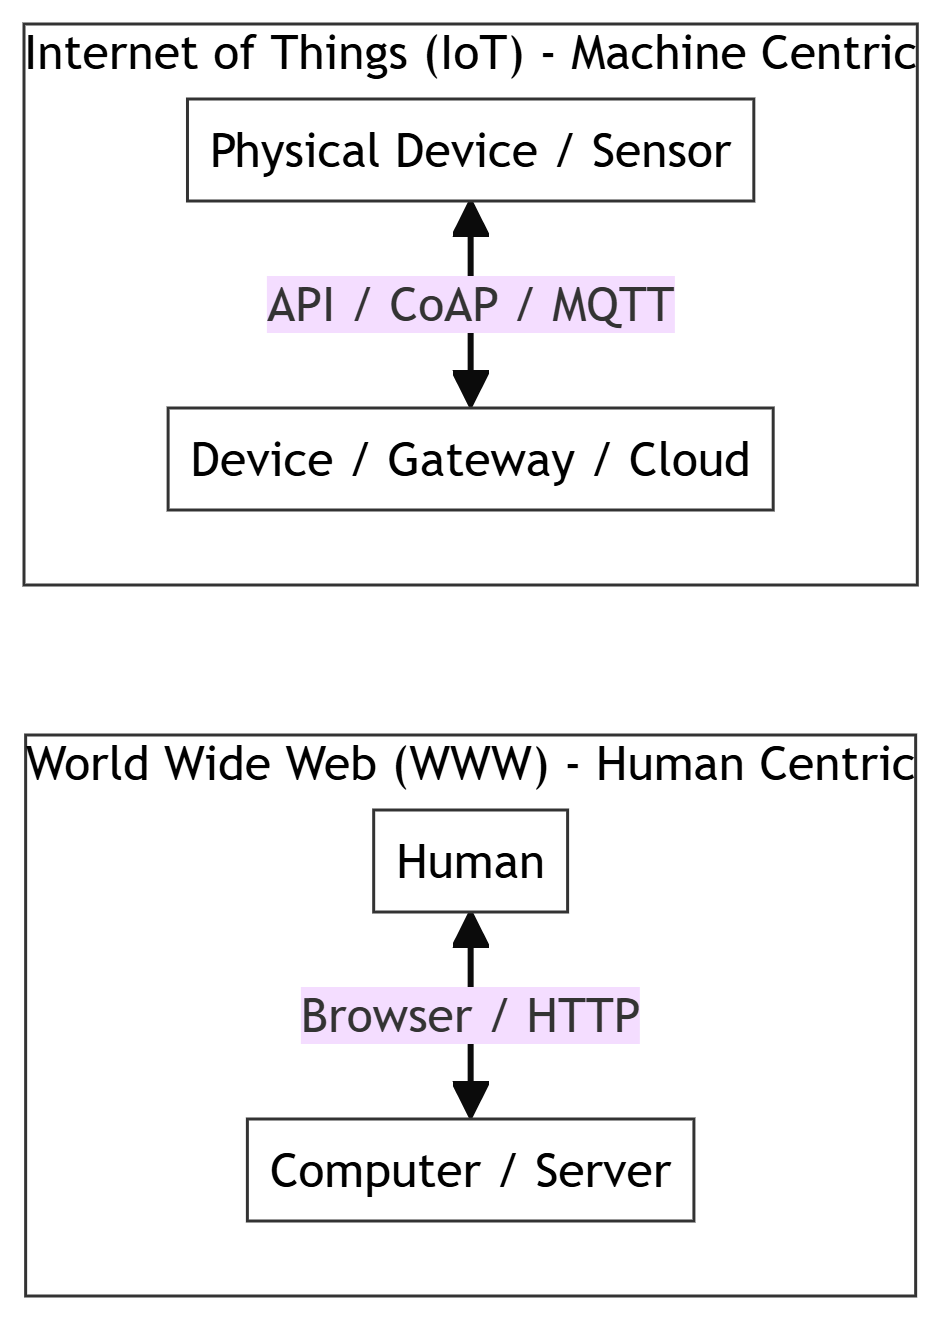
\includegraphics[width=0.75\textwidth,height=0.32\textheight,keepaspectratio]{../Images/chapter_01/www_vs_iot.png}
\caption{WWW vs. IoT Comparison}
\end{figure}

\subsection{3. Four Primary Application Areas}
\begin{enumerate}
  \item \textbf{Consumer / Smart Home:} Smart thermostats (e.g., Nest), connected lighting (e.g., Philips Hue), and home security systems.
  \item \textbf{Industrial IoT (IIoT):} Predictive maintenance of machinery, supply chain asset tracking, and smart factory automation.
  \item \textbf{Healthcare:} Wearable health trackers, remote patient monitoring devices, and smart pill bottles.
  \item \textbf{Smart Infrastructure:} Intelligent transportation systems, smart electrical grids, and automatic environmental tracking (pollution/weather).
\end{enumerate}


\section{Section 2: WSN, M2M and IoT Comparison (Q1.2)}

\subsection{1. Wireless Sensor Network (WSN) vs. IoT}
\begin{itemize}
  \item   \textbf{Wireless Sensor Network (WSN):} A localized network of spatially distributed autonomous devices (nodes) equipped with sensors to monitor physical or environmental conditions (e.g., temperature, pressure). WSNs focus on \textbf{data collection} and sending it to a central sink node; they typically lack direct internet connectivity or actuators to affect the environment.
  \item   \textbf{Internet of Things (IoT):} A global network that integrates WSNs, actuators, internet connectivity, cloud storage, and analytics. While WSNs only sense the world, IoT systems can \textbf{sense, think, and act} by feeding data to actuators to dynamically modify the environment.
\end{itemize}

\subsection{2. M2M vs. IoT Characteristics}

\begin{table}[H]
\centering
\begin{tabular}{|p{\dimexpr 0.2\textwidth - 2\tabcolsep - 1.5\arrayrulewidth\relax}|p{\dimexpr 0.4\textwidth - 2\tabcolsep - 1.5\arrayrulewidth\relax}|p{\dimexpr 0.4\textwidth - 2\tabcolsep - 1.5\arrayrulewidth\relax}|}
\hline
Feature / Criteria & Machine-to-Machine (M2M) & Internet of Things (IoT) \\
\hline
\textbf{Scope of Connectivity} & Point-to-point, closed system (usually localized or cellular). & Global network, open standard internet protocols. \\
\hline
\textbf{Communication Type} & Device-to-device (usually direct, isolated links). & Device-to-device, Device-to-Cloud, and Cloud-to-Cloud. \\
\hline
\textbf{Hardware Focus} & Hardware-centric (focused on physical machine links). & Software \& Data-centric (focused on API integration and analytics). \\
\hline
\textbf{Standards \& Protocols} & Proprioceptive or legacy protocols (cellular/proprietary). & Open internet protocols (IP, TCP/IP, MQTT, CoAP). \\
\hline
\textbf{Value Focus} & Operational efficiency (monitoring single machine states). & Business transformation (big data analytics, value-driven chains). \\
\hline
\end{tabular}
\end{table}


\section{Section 3: Flavors, Enchanted Objects and Creators (Q1.8)}

\subsection{1. The Concept of an "Enchanted Object"}
Coined by David Rose, an \textbf{Enchanted Object} is a physical, everyday item that has been digitally enhanced with sensors, actuators, and internet connectivity, giving it extraordinary capabilities while maintaining its original, intuitive physical form.
\begin{itemize}
  \item   \textbf{Example:} A standard umbrella handle that glows blue when the local weather report forecasts rain. It does not force the user to look at a smartphone screen; instead, it uses subtle, ambient cues to deliver information.
\end{itemize}

\subsection{2. The Four "Flavors" (Architectures) of IoT Communication}
\begin{enumerate}
  \item \textbf{Device-to-Device (D2D):} Two or more devices communicate directly with each other over local, short-range wireless links (e.g., Bluetooth, Zigbee) without routing data through an internet server.
  \item \textbf{Device-to-Cloud (D2C):} An IoT device connects directly to an internet cloud service (e.g., AWS IoT, Azure) using standard protocols like IP/TCP to upload data and receive control commands.
  \item \textbf{Device-to-Gateway (D2G / Gateway):} Constraint devices connect to an intermediate \textbf{gateway node} over local protocols. The gateway translates protocols, aggregates data, and forwards it to the internet cloud.
  \item \textbf{Back-End Data Sharing (C2C / Cloud-to-Cloud):} Cloud services communicate with other cloud databases via Web APIs (REST/JSON), allowing third-party services to share and analyze aggregated device data.
\end{enumerate}

\subsection{3. Categories of IoT Creators}
\begin{itemize}
  \item   \textbf{Makers \& Hobbyists:} Use open-source platforms (Arduino, Raspberry Pi) to build custom home hacks and rapid, low-cost prototypes.
  \item   \textbf{Startups:} Focus on rapid market entry, using lean principles to launch niche consumer or enterprise products.
  \item   \textbf{Industrial Engineers:} Focus on operational efficiency, retrofitting legacy industrial machines with modern smart sensors.
  \item   \textbf{Corporate Developers \& Enterprise Architects:} Build scalable, highly secure corporate cloud platforms to handle millions of streaming data connections.
\end{itemize}


\section{Section 4: M2M vs. IoT Health Band Case Study (Q1.3)}

To illustrate the potential and benefits of an IoT-oriented approach over traditional M2M, let us compare their deployment in a wearable \textbf{Health Band}:

\subsection{1. The M2M Approach}
\begin{itemize}
  \item   \textbf{Architecture:} The health band uses a cellular transmitter to send a user's heart rate directly to a doctor's monitor in a closed hospital network.
  \item   \textbf{Characteristics:}
\end{itemize}
    \textit{   }Isolated:* Only sends raw sensor data.
    \textit{   }No Integration:* The data cannot be accessed by other systems (e.g., the user's fitness apps, local pharmacies).
    \textit{   }No Scale:* Limited to a point-to-point connection.

\subsection{2. The IoT Approach}
\begin{itemize}
  \item   \textbf{Architecture:} The health band connects to the user's smartphone via Bluetooth Low Energy (BLE), which acts as a gateway to upload the data to an internet cloud.
  \item   \textbf{Characteristics \& Benefits:}
\end{itemize}
    \textit{   }Integration:* The data is shared via APIs with fitness trackers, calorie counter apps, and the user's electronic medical record (EMR).
    \textit{   }Edge \& Cloud Analytics:* The phone calculates immediate warnings locally, while the cloud performs predictive analytics on historical trends to warn of potential heart issues.
    \textit{   }Scalability:* Updates can be pushed to the device firmware over-the-air (OTA).


\section{Section 5: Standard Architectural Models (Q1.4, Q1.5, Q1.6, Q1.7)}

\subsection{1. ETSI M2M Functional Architecture}
The \textbf{European Telecommunications Standards Institute (ETSI)} defines a standardized, highly modular functional architecture for M2M communication:

\begin{figure}[H]
\centering
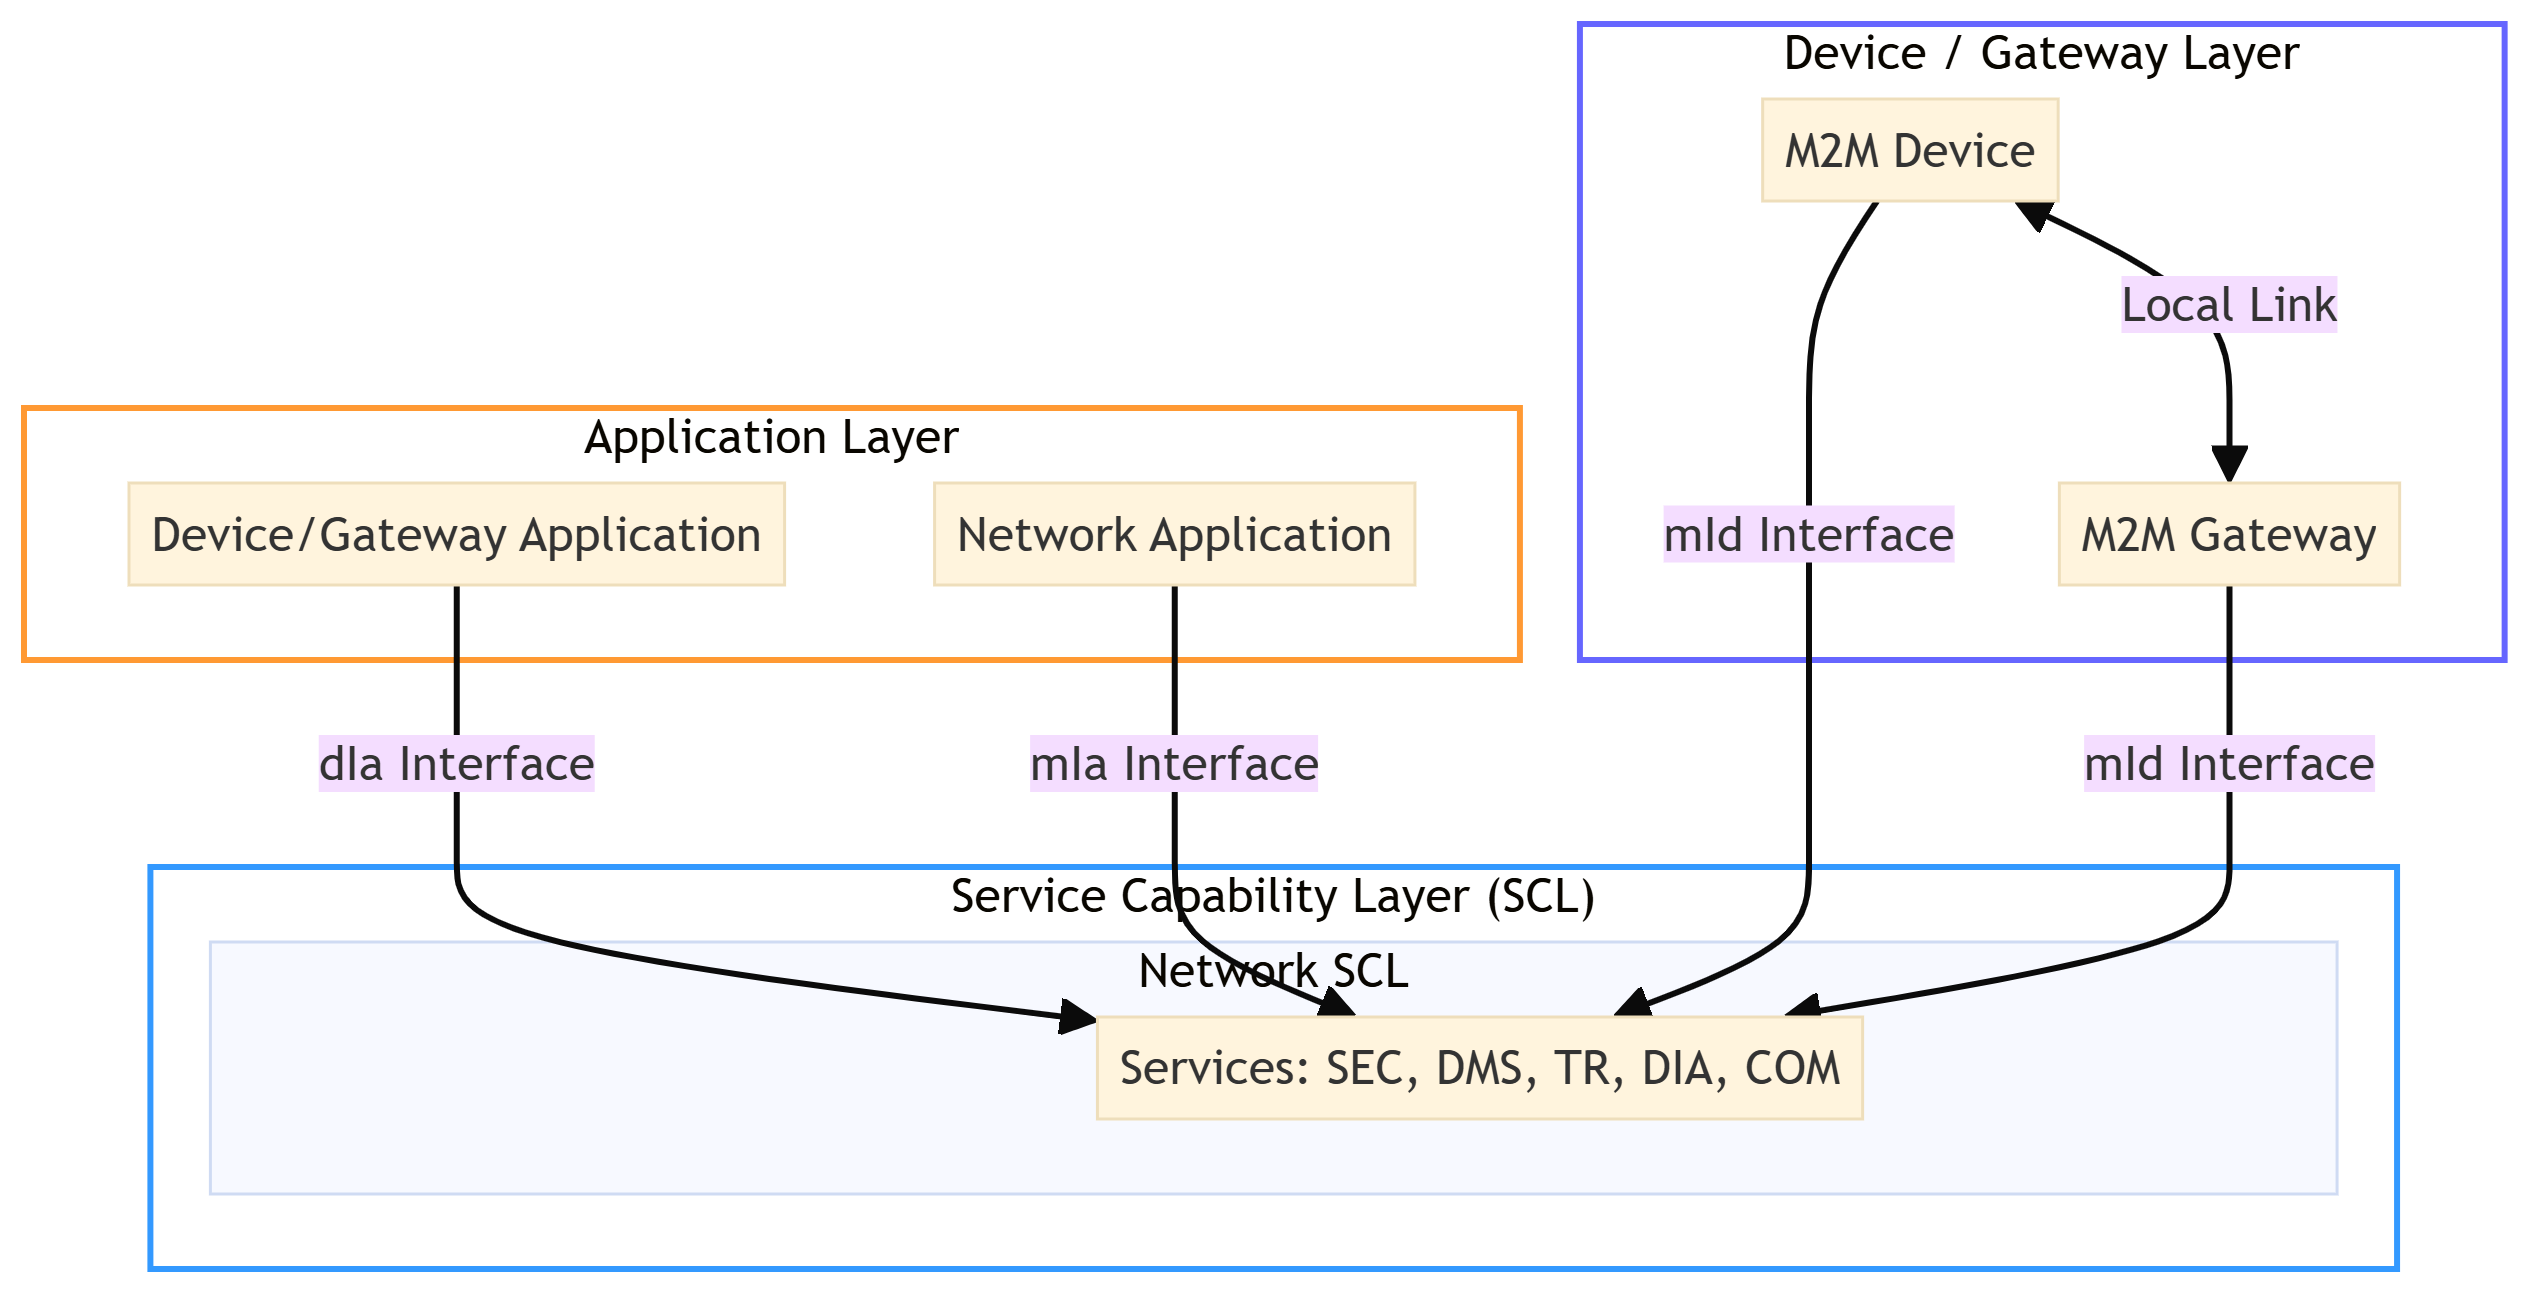
\includegraphics[width=0.75\textwidth,height=0.32\textheight,keepaspectratio]{../Images/chapter_01/etsi_m2m_architecture.png}
\caption{ETSI M2M Functional Architecture}
\end{figure}

\subsubsection{Three Core Interfaces:}
\begin{enumerate}
  \item \textbf{dIa (Device-to-Application):} Connects device applications to the local service capability layer.
  \item \textbf{mIa (M2M-to-Application):} Connects network applications to the network service capability layer.
  \item \textbf{mId (M2M-to-Device):} Connects the device/gateway layer to the network service capability layer.
\end{enumerate}

\subsubsection{Key Service Capabilities:}
\begin{itemize}
  \item   \textbf{SEC (Security):} Handles authentication and key management.
  \item   \textbf{DMS (Device Management):} Handles diagnostics and firmware updates.
  \item   \textbf{TR (Transaction Management):} Manages reliable data storage and queuing.
\end{itemize}


\subsection{2. OGC Functional Architecture}
The \textbf{Open Geospatial Consortium (OGC)} Sensor Web Enablement (SWE) framework focuses on making sensors discoverable and accessible over the web:

\begin{figure}[H]
\centering
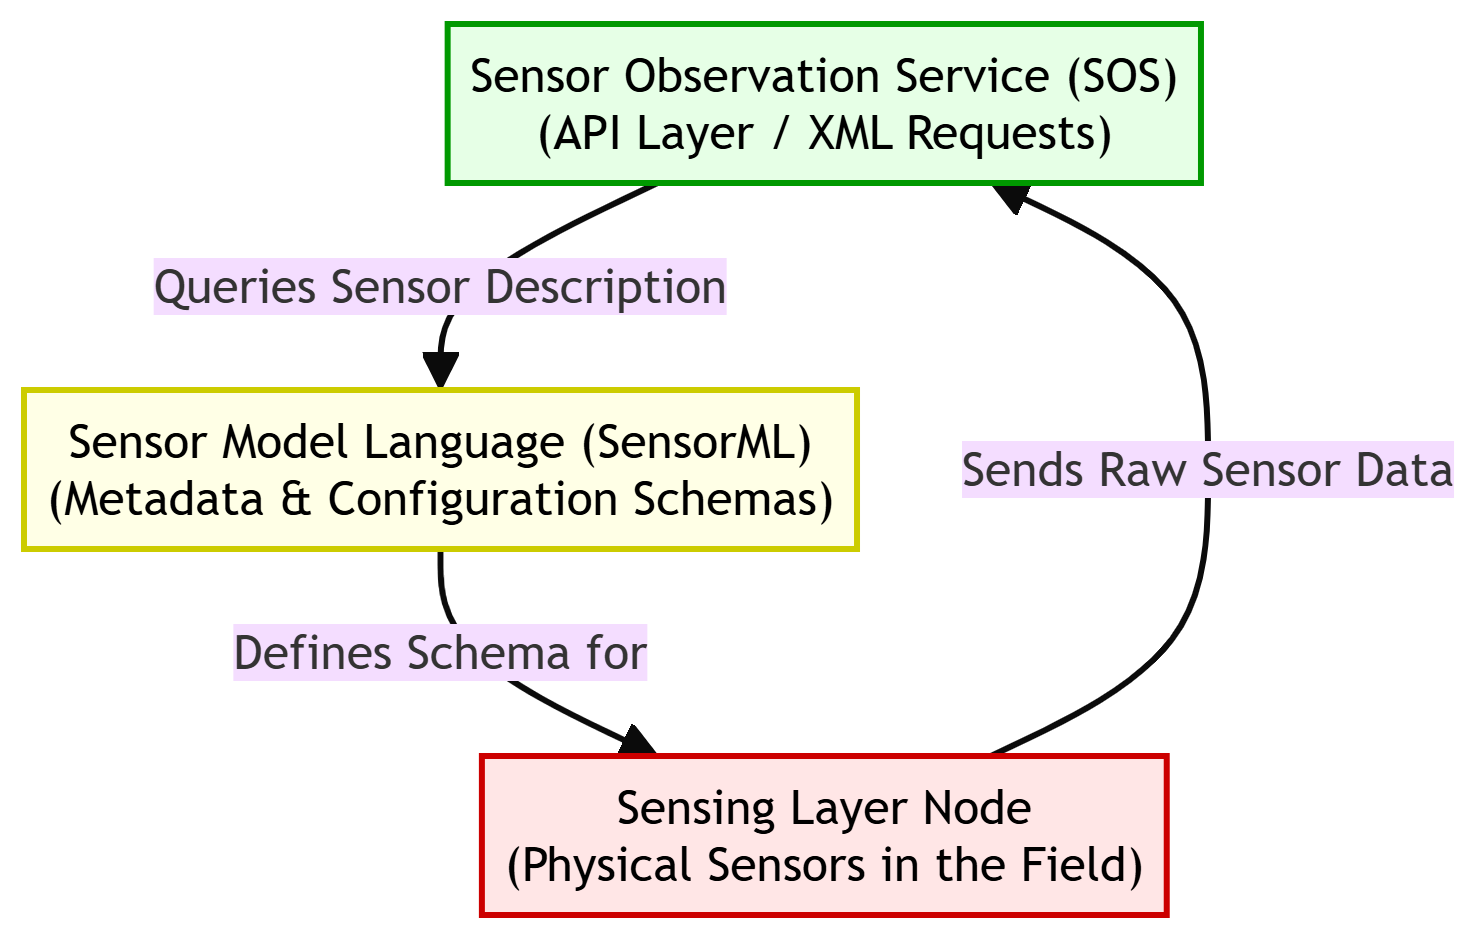
\includegraphics[width=0.75\textwidth,height=0.32\textheight,keepaspectratio]{../Images/chapter_01/ogc_architecture.png}
\caption{OGC Functional Architecture}
\end{figure}

\begin{itemize}
  \item   \textbf{Sensor Observation Service (SOS):} An API allowing clients to query real-time sensor observations.
  \item   \textbf{SensorML (Sensor Model Language):} An XML schema describing the metadata, parameters, and processing pipelines of the sensor systems.
\end{itemize}


\subsection{3. Generic M2M System Solution Functional Layers}
A complete end-to-end M2M system is composed of three main functional blocks:

\begin{enumerate}
  \item \textbf{M2M Area Network (Device Domain):} Comprises the sensors, actuators, and the local connectivity (e.g., Zigbee, Bluetooth, I2C bus) linking them to a local gateway.
  \item \textbf{Communication Network (Network Domain):} The bridge network carrying data across long distances (e.g., Cellular GSM/3G/4G, Wi-Fi, Ethernet, satellite).
  \item \textbf{M2M Applications (Application Domain):} The cloud backend where data is analyzed, databases are updated, and users view dashboards.
\end{enumerate}


\subsection{4. Information-Driven Value Chain}
The \textbf{Information-Driven Value Chain} maps how raw sensor measurements are transformed into valuable business decisions:

\begin{figure}[H]
\centering
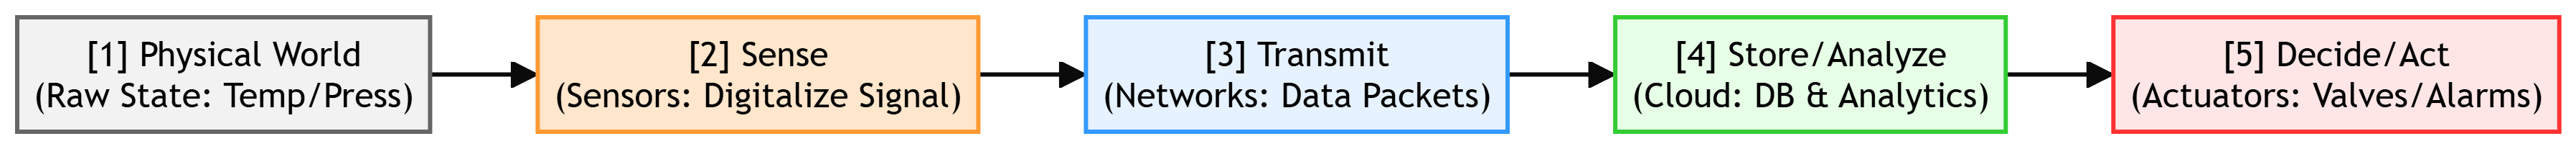
\includegraphics[width=0.75\textwidth,height=0.32\textheight,keepaspectratio]{../Images/chapter_01/information_value_chain.png}
\caption{Information-Driven Value Chain}
\end{figure}

\begin{enumerate}
  \item \textbf{Sense:} Sensors capture physical changes and convert them into electrical signals.
  \item \textbf{Transmit:} Wireless/wired modules send the digitized measurements across IP networks.
  \item \textbf{Store/Analyze:} Databases store the historical logs while analytics software processes the streams for anomalies.
  \item \textbf{Decide/Act:} Actuators execute control actions (e.g., shutting down a motor, opening a valve) based on the analytical findings.
\end{enumerate}


\section{Section 6: Supplemental Exam Topics}

\subsection{1. Top Challenges of Implementing an IoT System}
\begin{itemize}
  \item   \textbf{Security \& Privacy:} Constrained devices lack the memory to run heavy encryption algorithms, leaving them open to hacking.
  \item   \textbf{Interoperability:} Gaps in standardized platforms cause communication silos between different manufacturers.
  \item   \textbf{Data Volume:} Managing and processing the massive streams of unstructured data generated by millions of sensors.
  \item   \textbf{Power Limits:} Many remote sensors run on small batteries and must survive for years without a battery change.
\end{itemize}

\subsection{2. IoT vs. Industrial IoT (IIoT)}
\begin{itemize}
  \item   \textbf{Internet of Things (IoT):} Typically consumer-oriented (e.g., smart home devices, health wearables). Focuses on \textbf{user convenience} and has moderate security and reliability requirements. A system crash is a minor inconvenience.
  \item   \textbf{Industrial IoT (IIoT):} Mission-critical industrial systems (e.g., power plants, manufacturing lines). Focuses on \textbf{system safety, zero downtime, and extreme reliability}. A system crash can lead to massive financial loss or loss of life.
\end{itemize}

\subsection{3. ICT Trends Affecting IoT}
\begin{itemize}
  \item   \textbf{Cloud to Edge Computing:} Shifting heavy analytics from centralized cloud databases to localized edge gateways to reduce communication latency.
  \item   \textbf{IPv4 to IPv6 Migration:} Providing a massive address space to accommodate billions of unique connected endpoints.
  \item   \textbf{Low-Power Wide-Area Networks (LPWAN):} Rise of cellular protocols like NB-IoT and LoRaWAN designed specifically for low-power, long-distance sensor nodes.
\end{itemize}
